\subsection{Cambios realizados sobre la primera entrega}

En el subsistema de música se han añadido requisitos correspondientes a las funciones de modificación y eliminación de canciones, autores y géneros.

En el subsistema de usuarios, ha sido necesario añadir un requisito de datos manejados para uno de los requisitos funcionales, ya que a la hora de realizar los refinamientos hemos visto que era necesario y durante la primera práctica no lo habiamos tenido en cuenta. En consecuencia, hay cambios en las tablas del final de la práctica.

\subsection{Esquema de caja negra}

\begin{figure}[H]
  \centering
  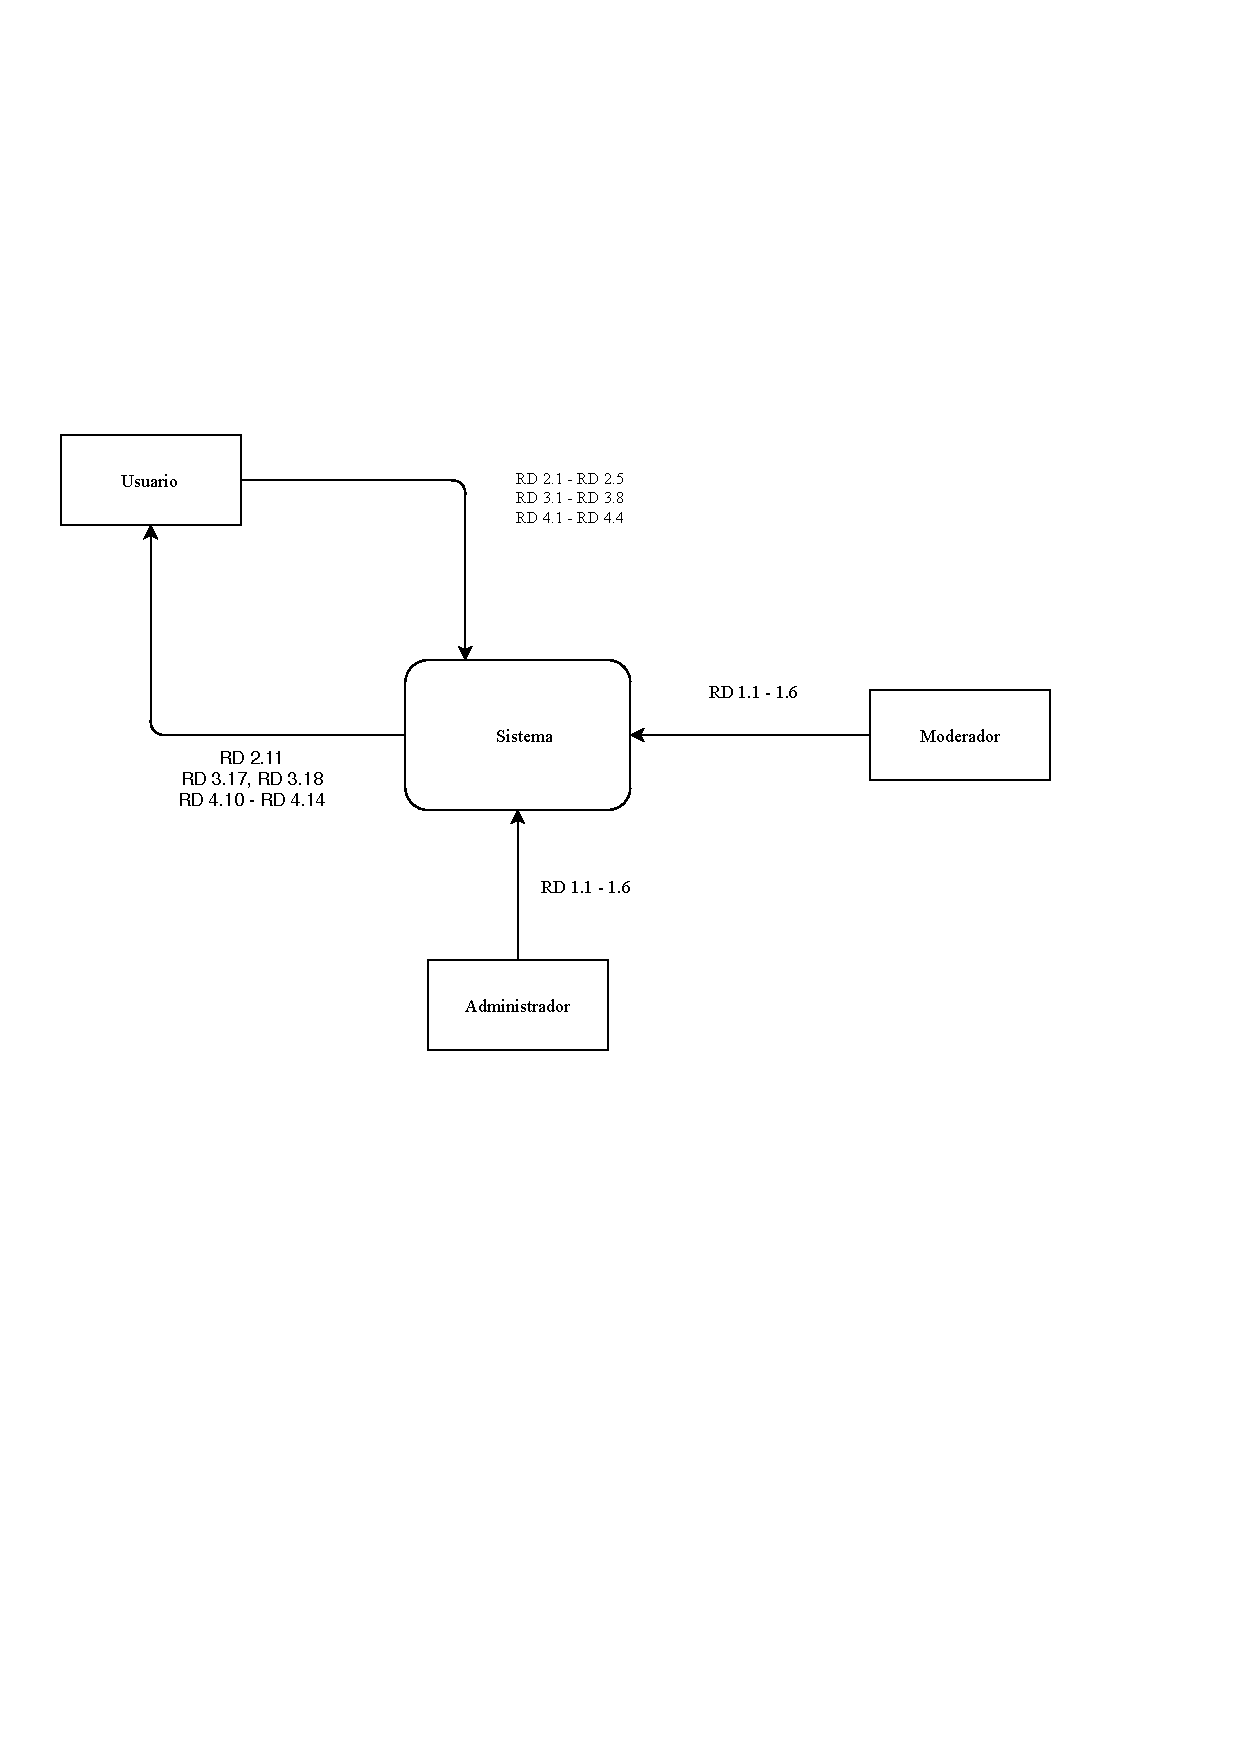
\includegraphics{diagramas/Caja_negra.pdf}
\end{figure}

\subsection{Esquema armazón}

\begin{figure}[H]
  \centering
  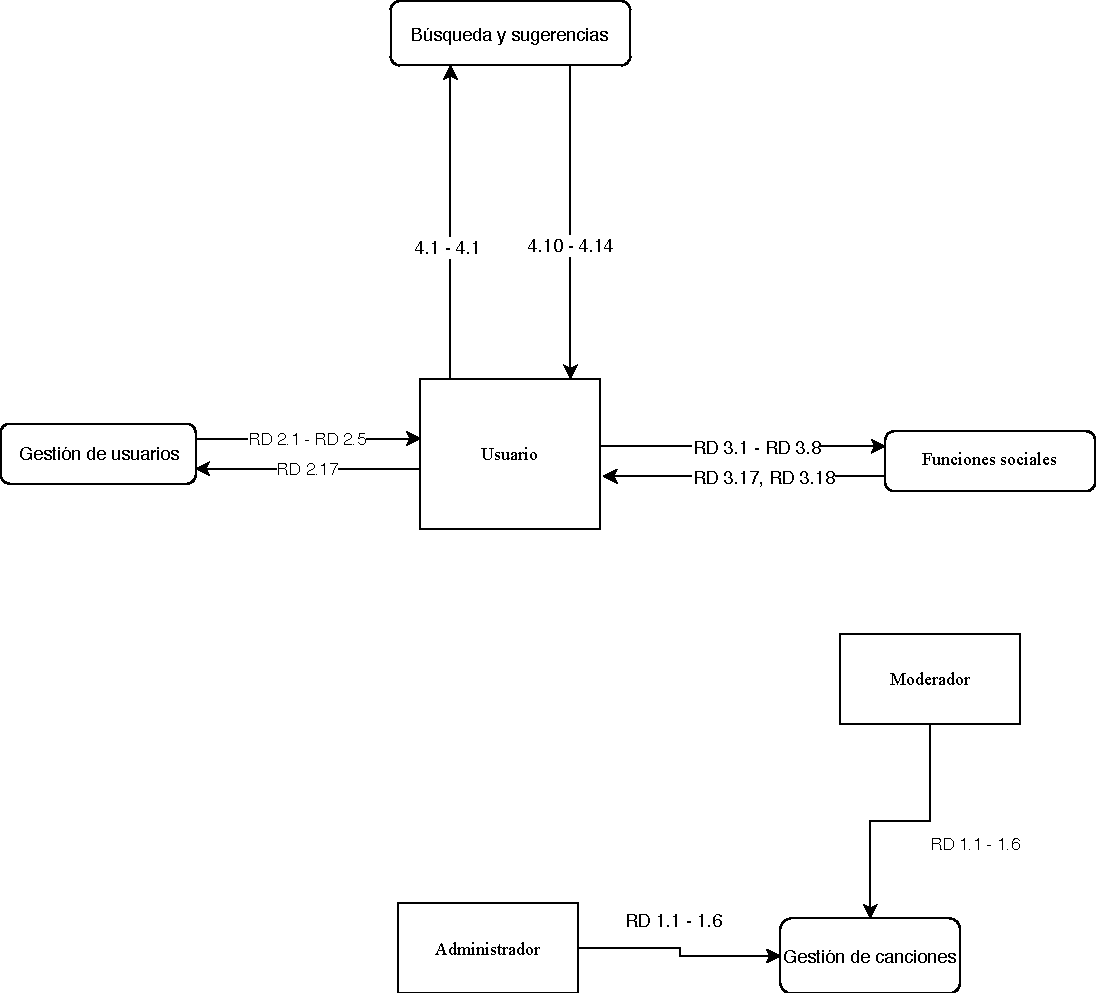
\includegraphics[scale=0.9]{diagramas/Esquema_armazon.pdf}
\end{figure}

\subsection{Refinamientos de los subsistemas}

\begin{figure}[H]
  \caption{Refinamiento del subsistema de música.}
  \centering
  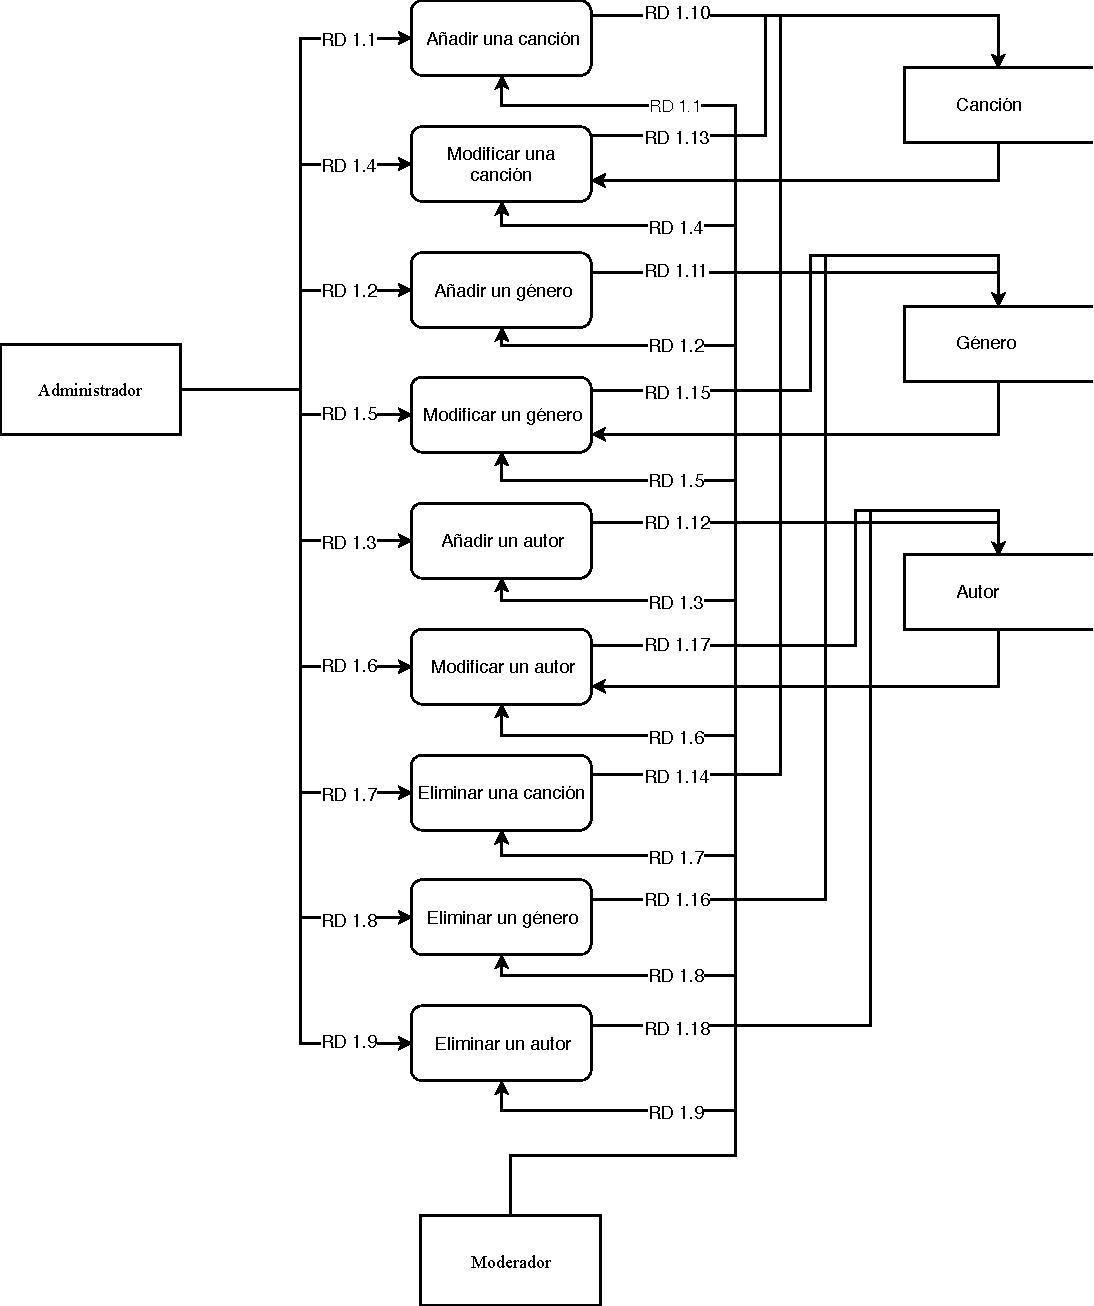
\includegraphics[scale=0.9]{diagramas/musica2.pdf}
\end{figure}

\begin{figure}[H]
  \caption{Refinamiento del subsistema de usuarios.}
  \centering
  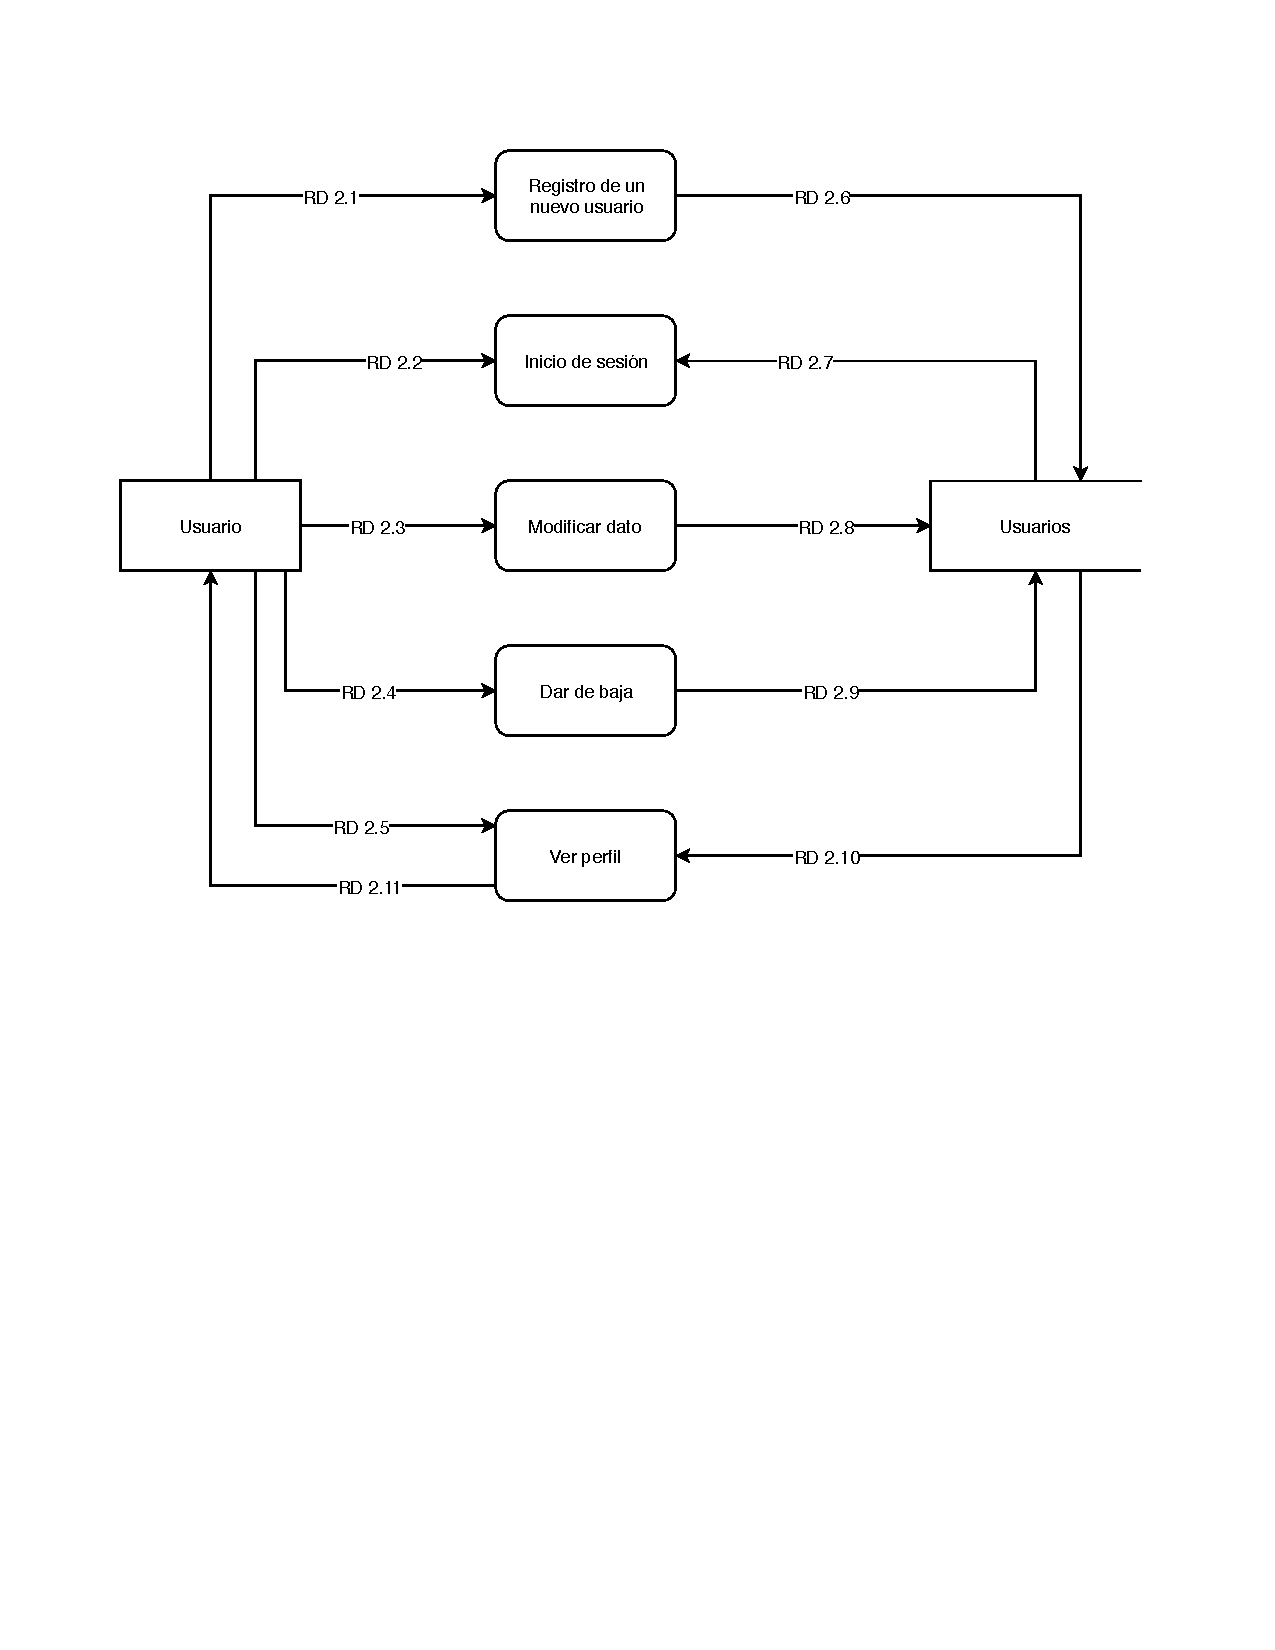
\includegraphics[scale=0.9]{diagramas/ref-usuario.pdf}
\end{figure}

\begin{figure}[H]
  \caption{Refinamiento del subsistema social}
  \centering
  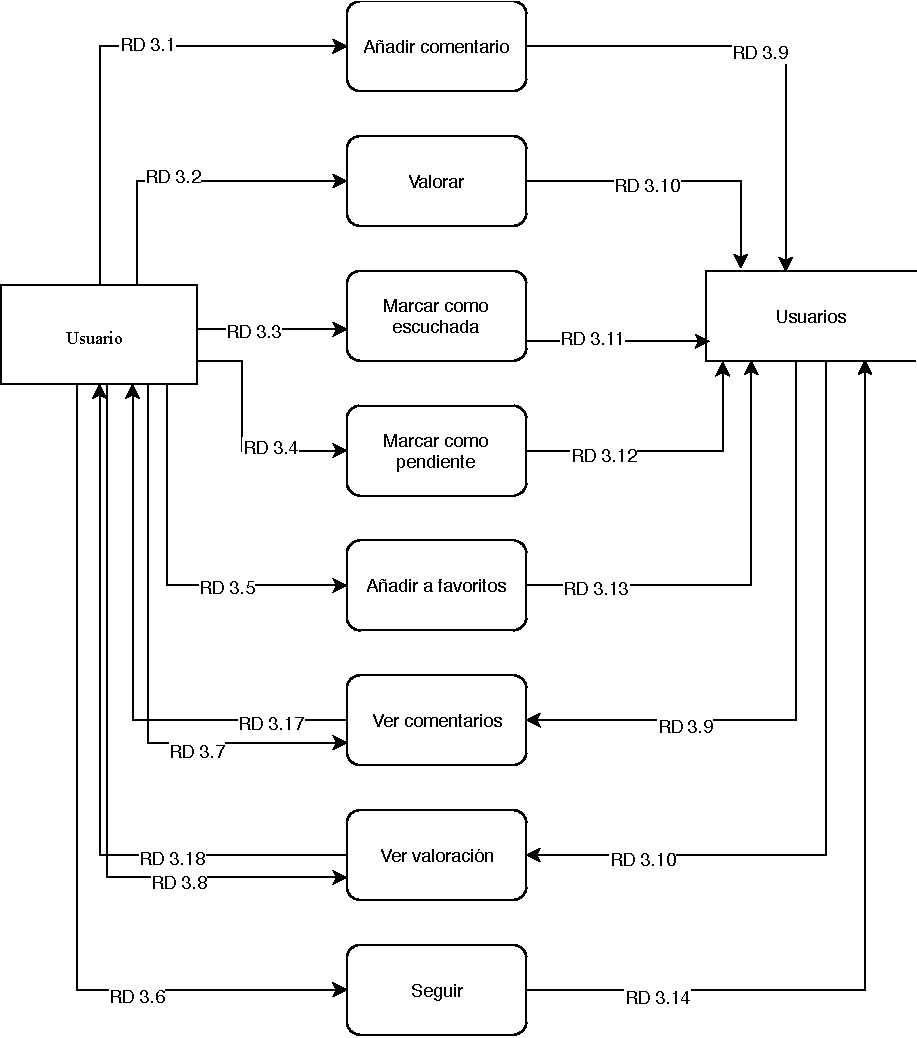
\includegraphics{diagramas/ref-social.pdf}
\end{figure}

\begin{figure}[H]
  \caption{Refinamiento del subsistema de búsquedas y sugerencias}
  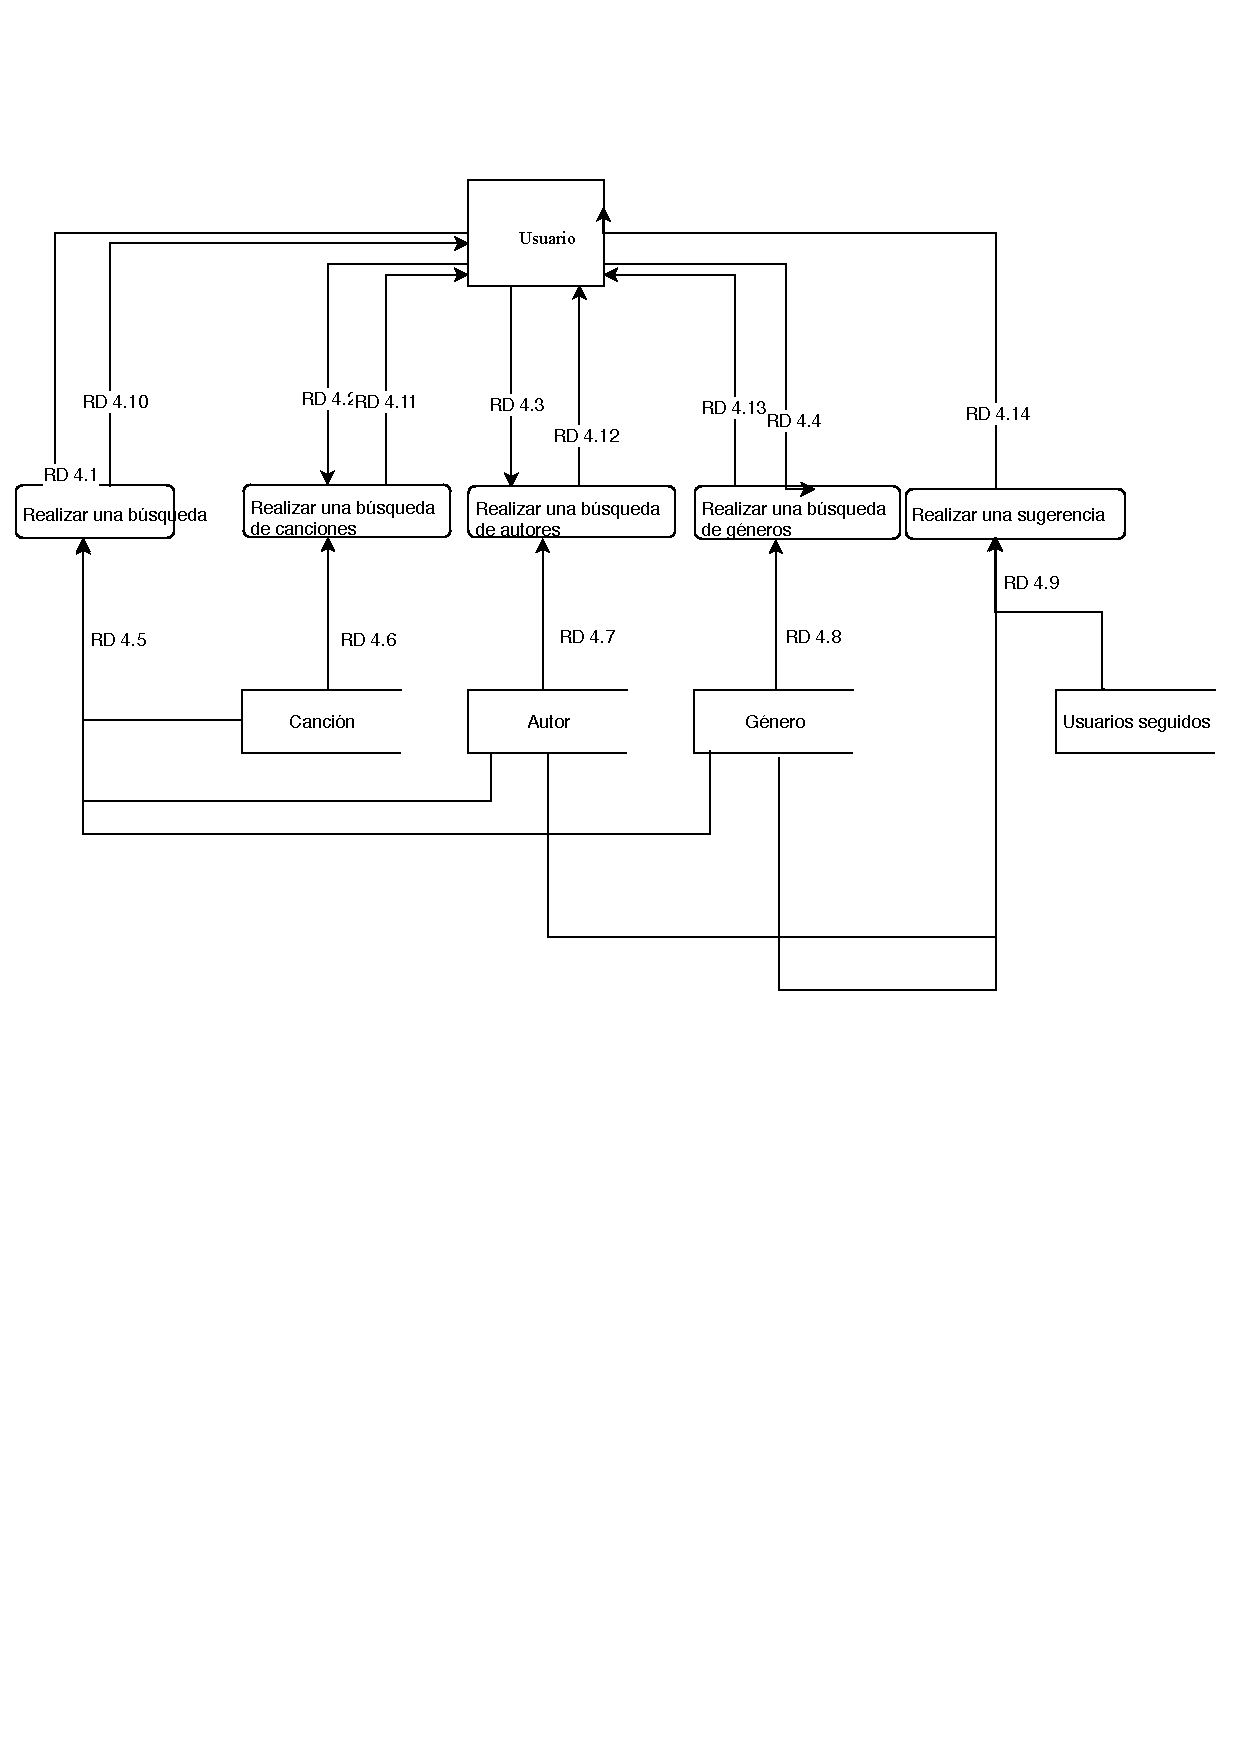
\includegraphics[scale=0.85]{diagramas/busqueda_refinamiento.pdf}
\end{figure}

\subsection{Esquemas externos}

\begin{figure}[H]
  \caption{Esquemas externos del subsistema de música - canciones}
  \centering
  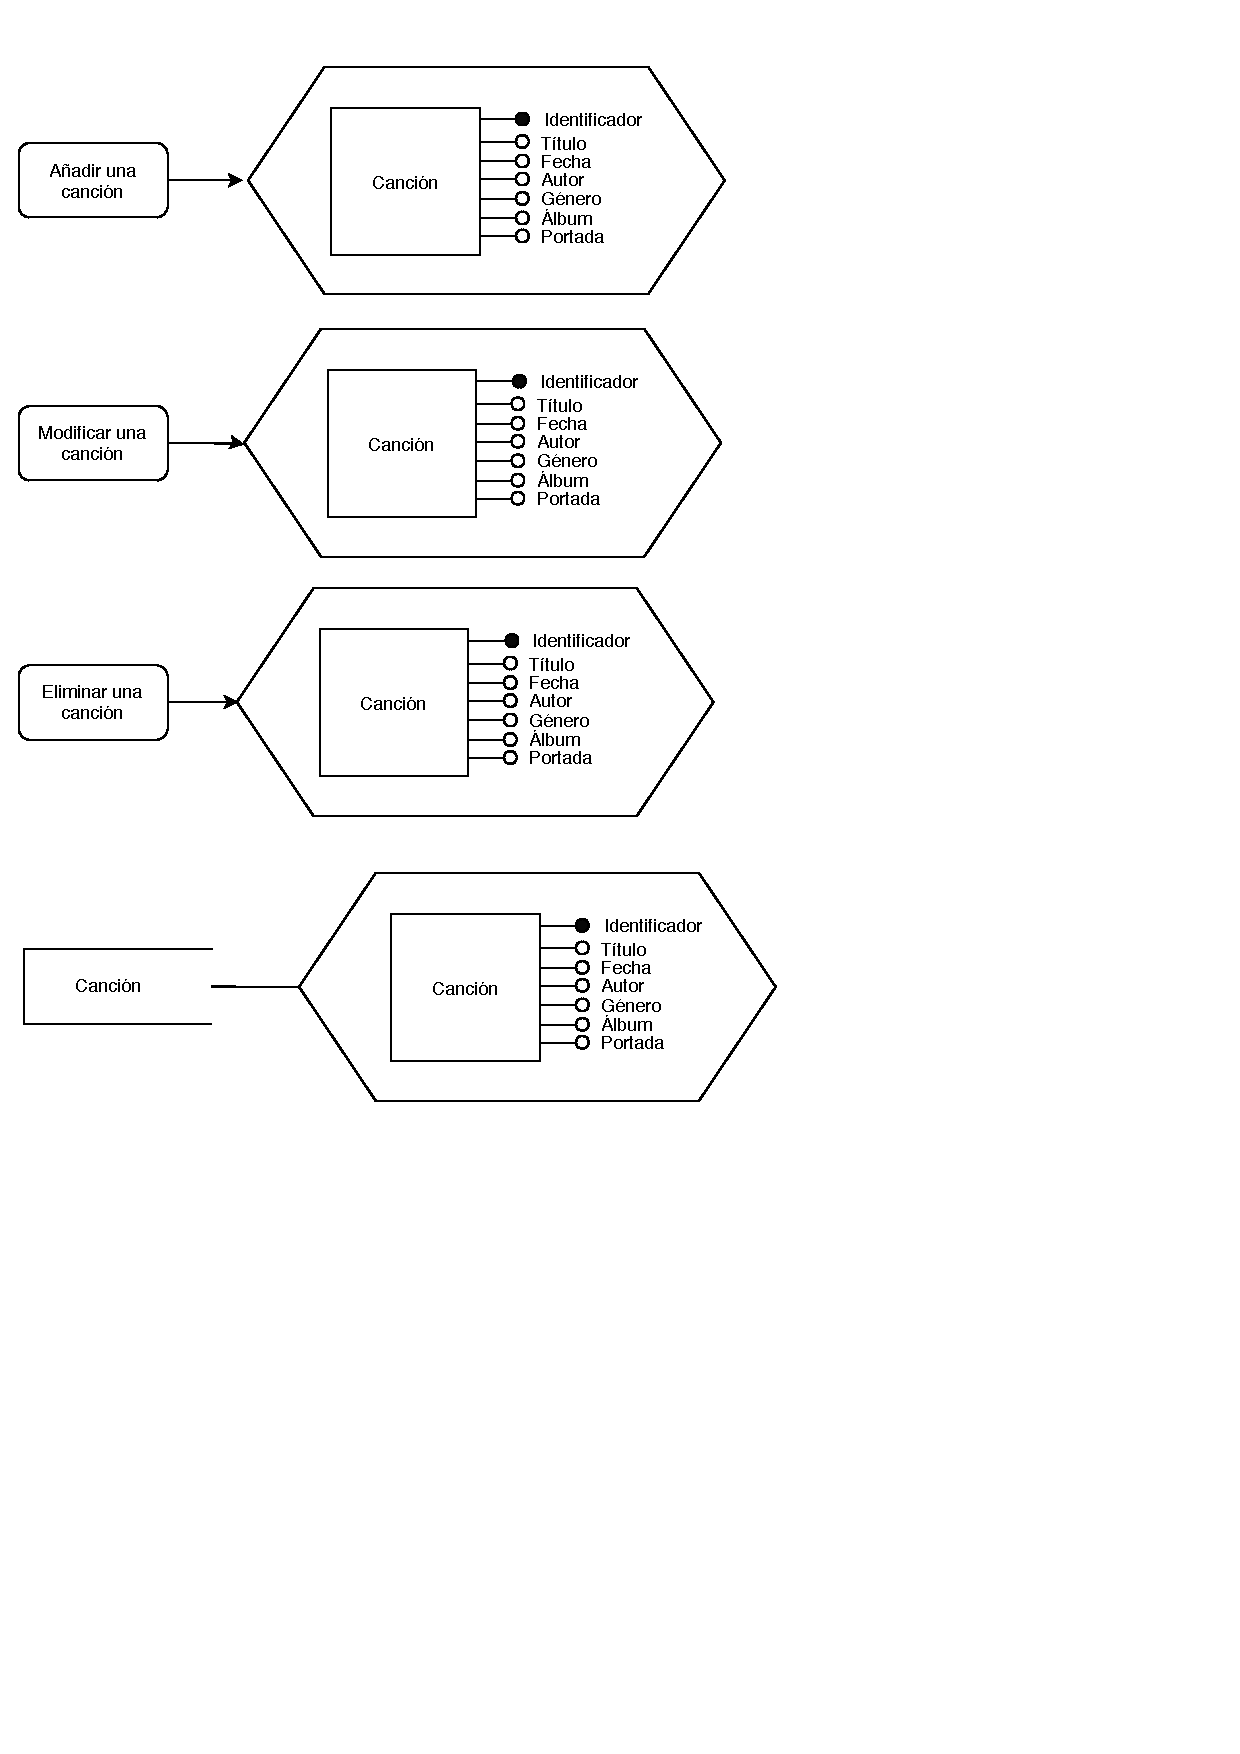
\includegraphics[scale=0.7]{diagramas/musica-externo-cancion.pdf}
\end{figure}

\begin{figure}[H]
  \caption{Esquemas externos del subsistema de música - autores}
  \centering
  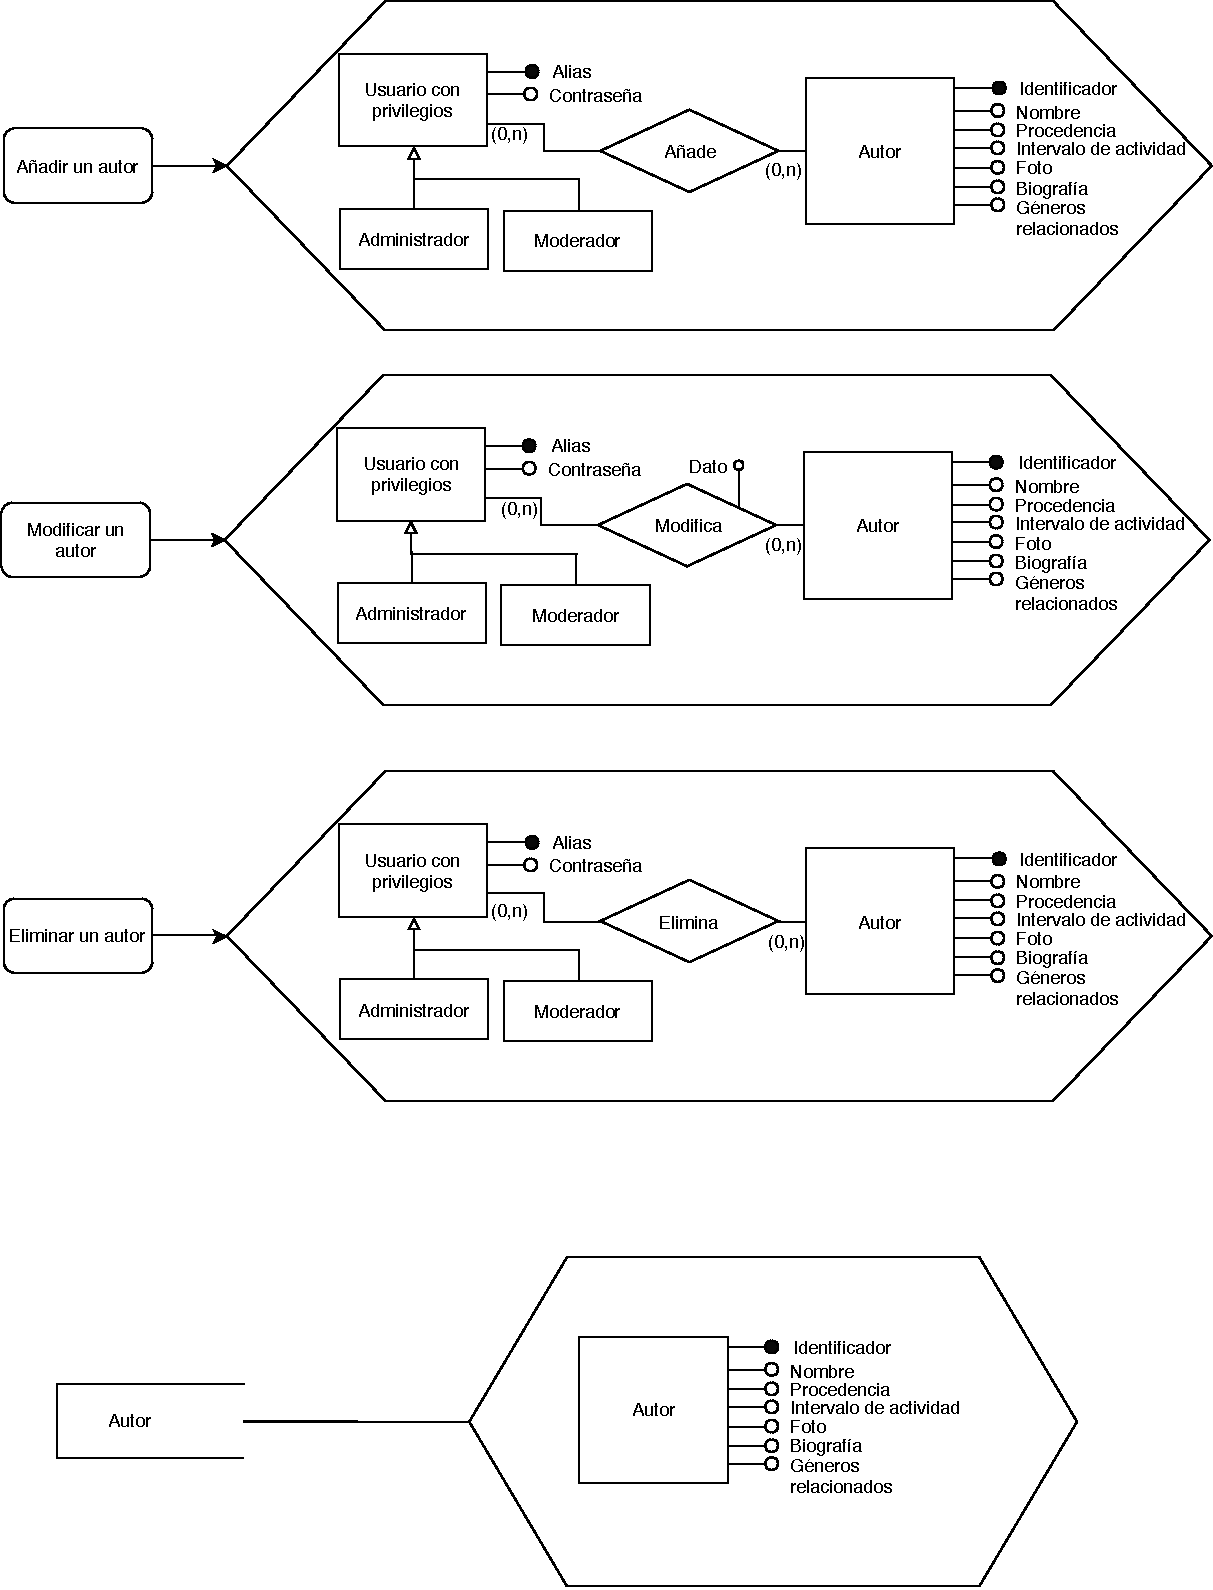
\includegraphics[scale=0.7]{diagramas/musica-externo-autor.pdf}
\end{figure}

\begin{figure}[H]
  \caption{Esquemas externos del subsistema de música - géneros}
  \centering
  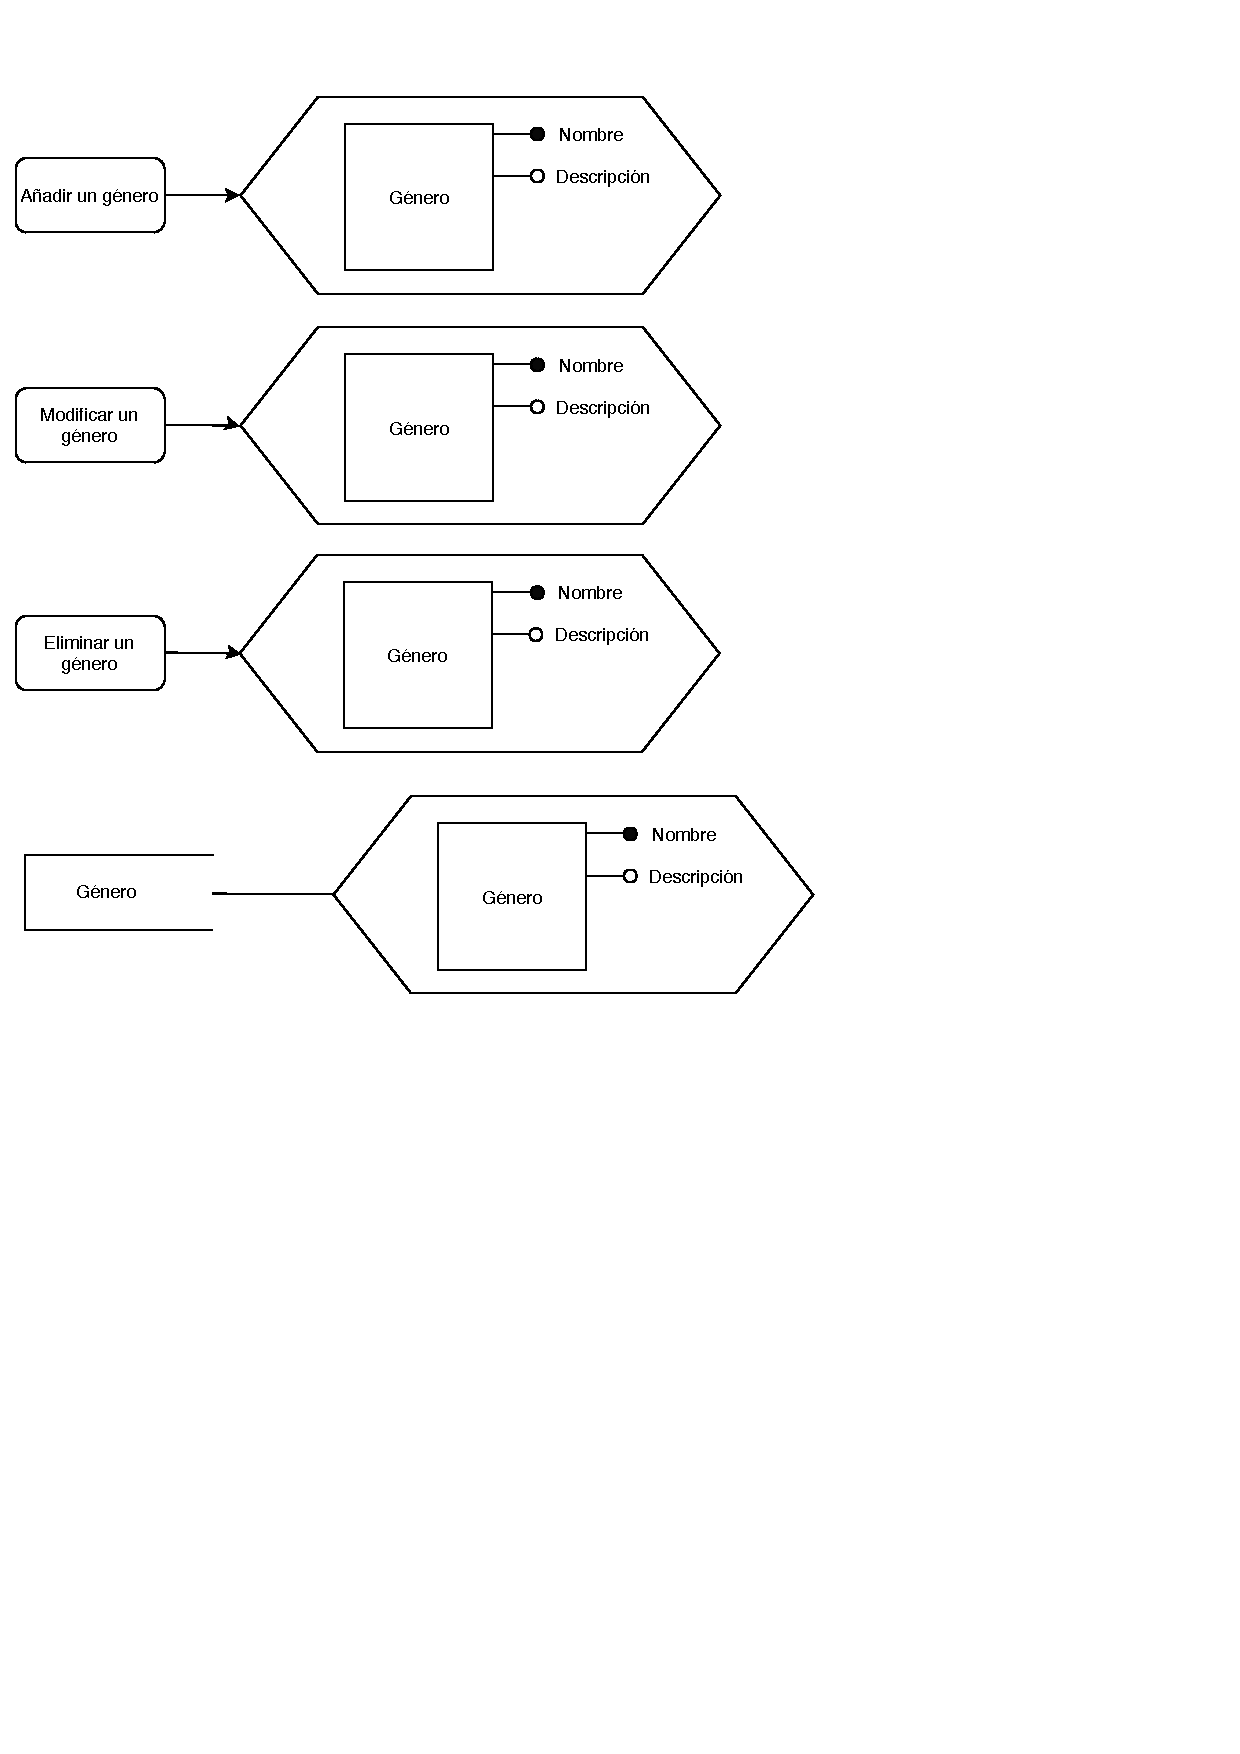
\includegraphics[scale=0.7]{diagramas/musica-externo-genero.pdf}
\end{figure}

\begin{figure}[H]
  \caption{Esquemas externos del subsistema de usuarios}
  \centering
  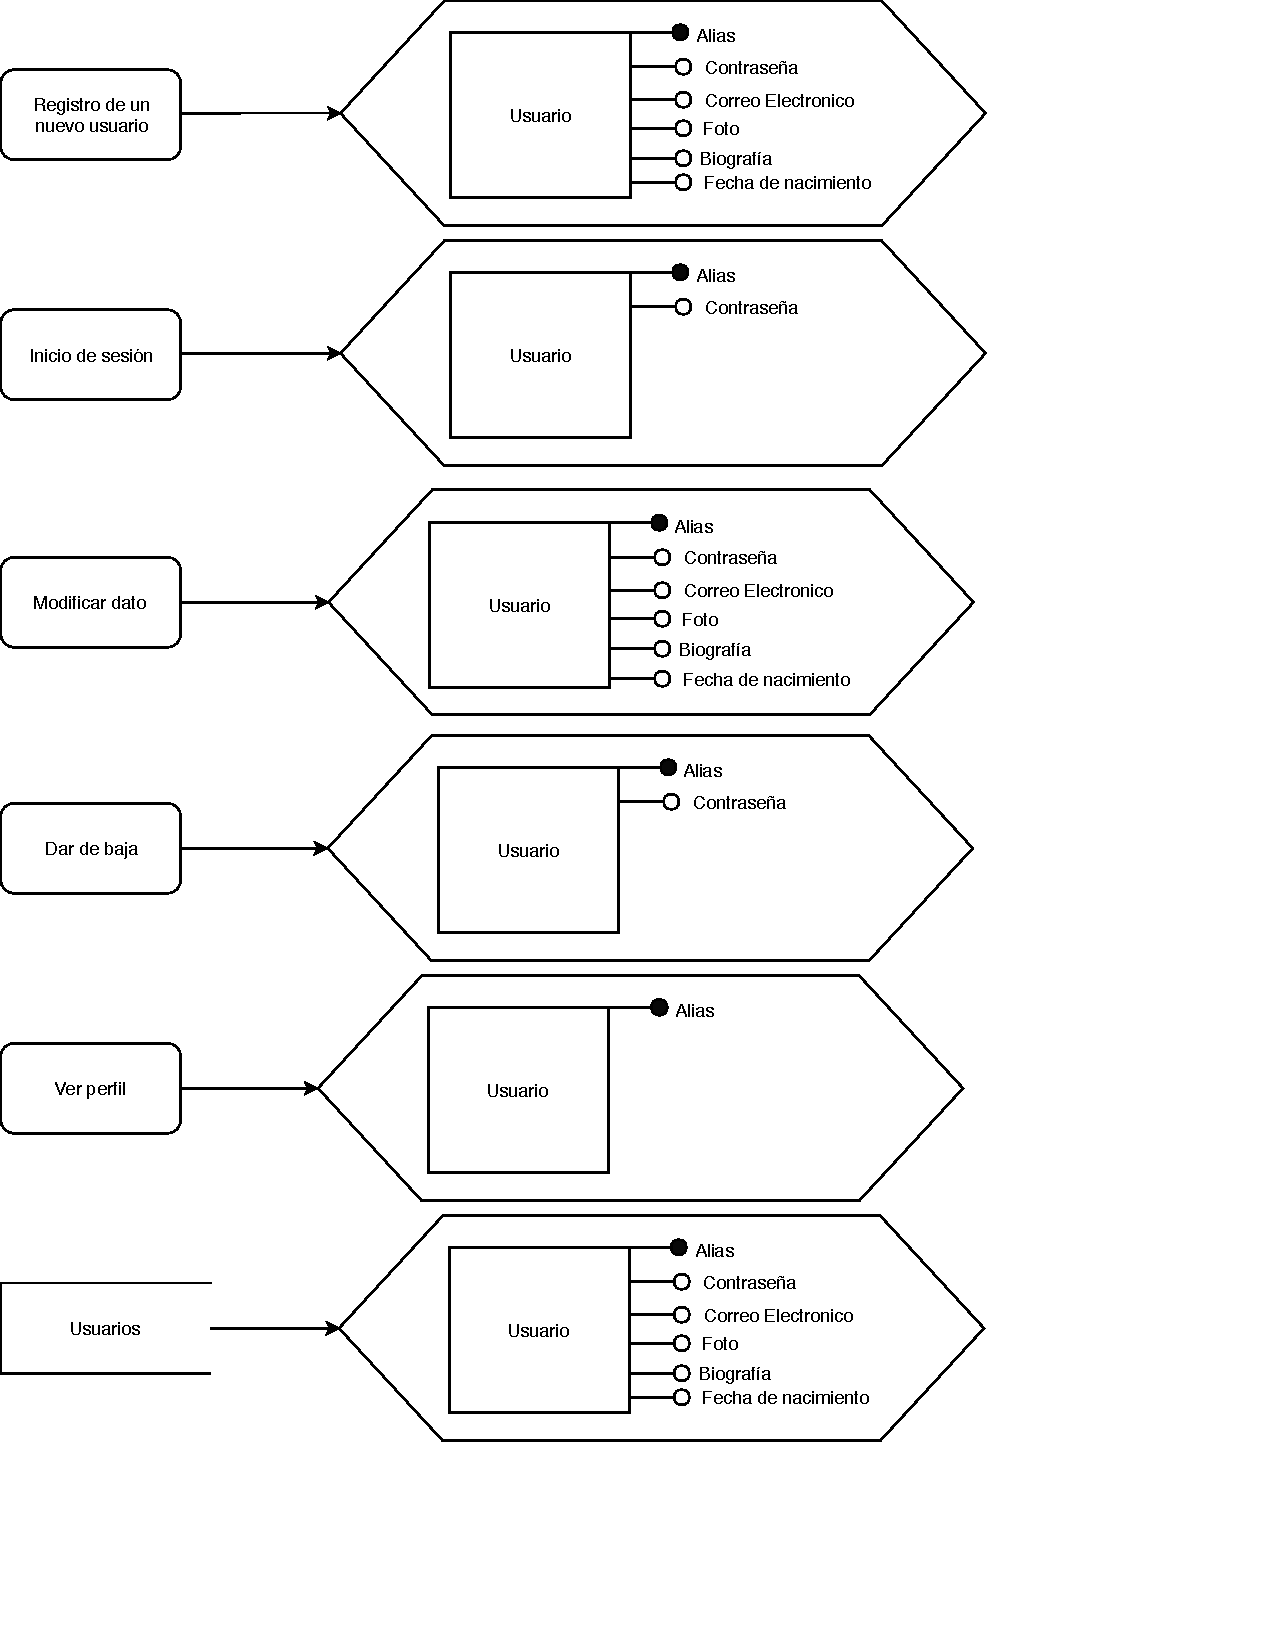
\includegraphics[scale=0.8]{diagramas/Esq-ext-usuario.pdf}
\end{figure}

\begin{figure}[H]
  \caption{Esquemas externos del subsistema social}
  \centering
  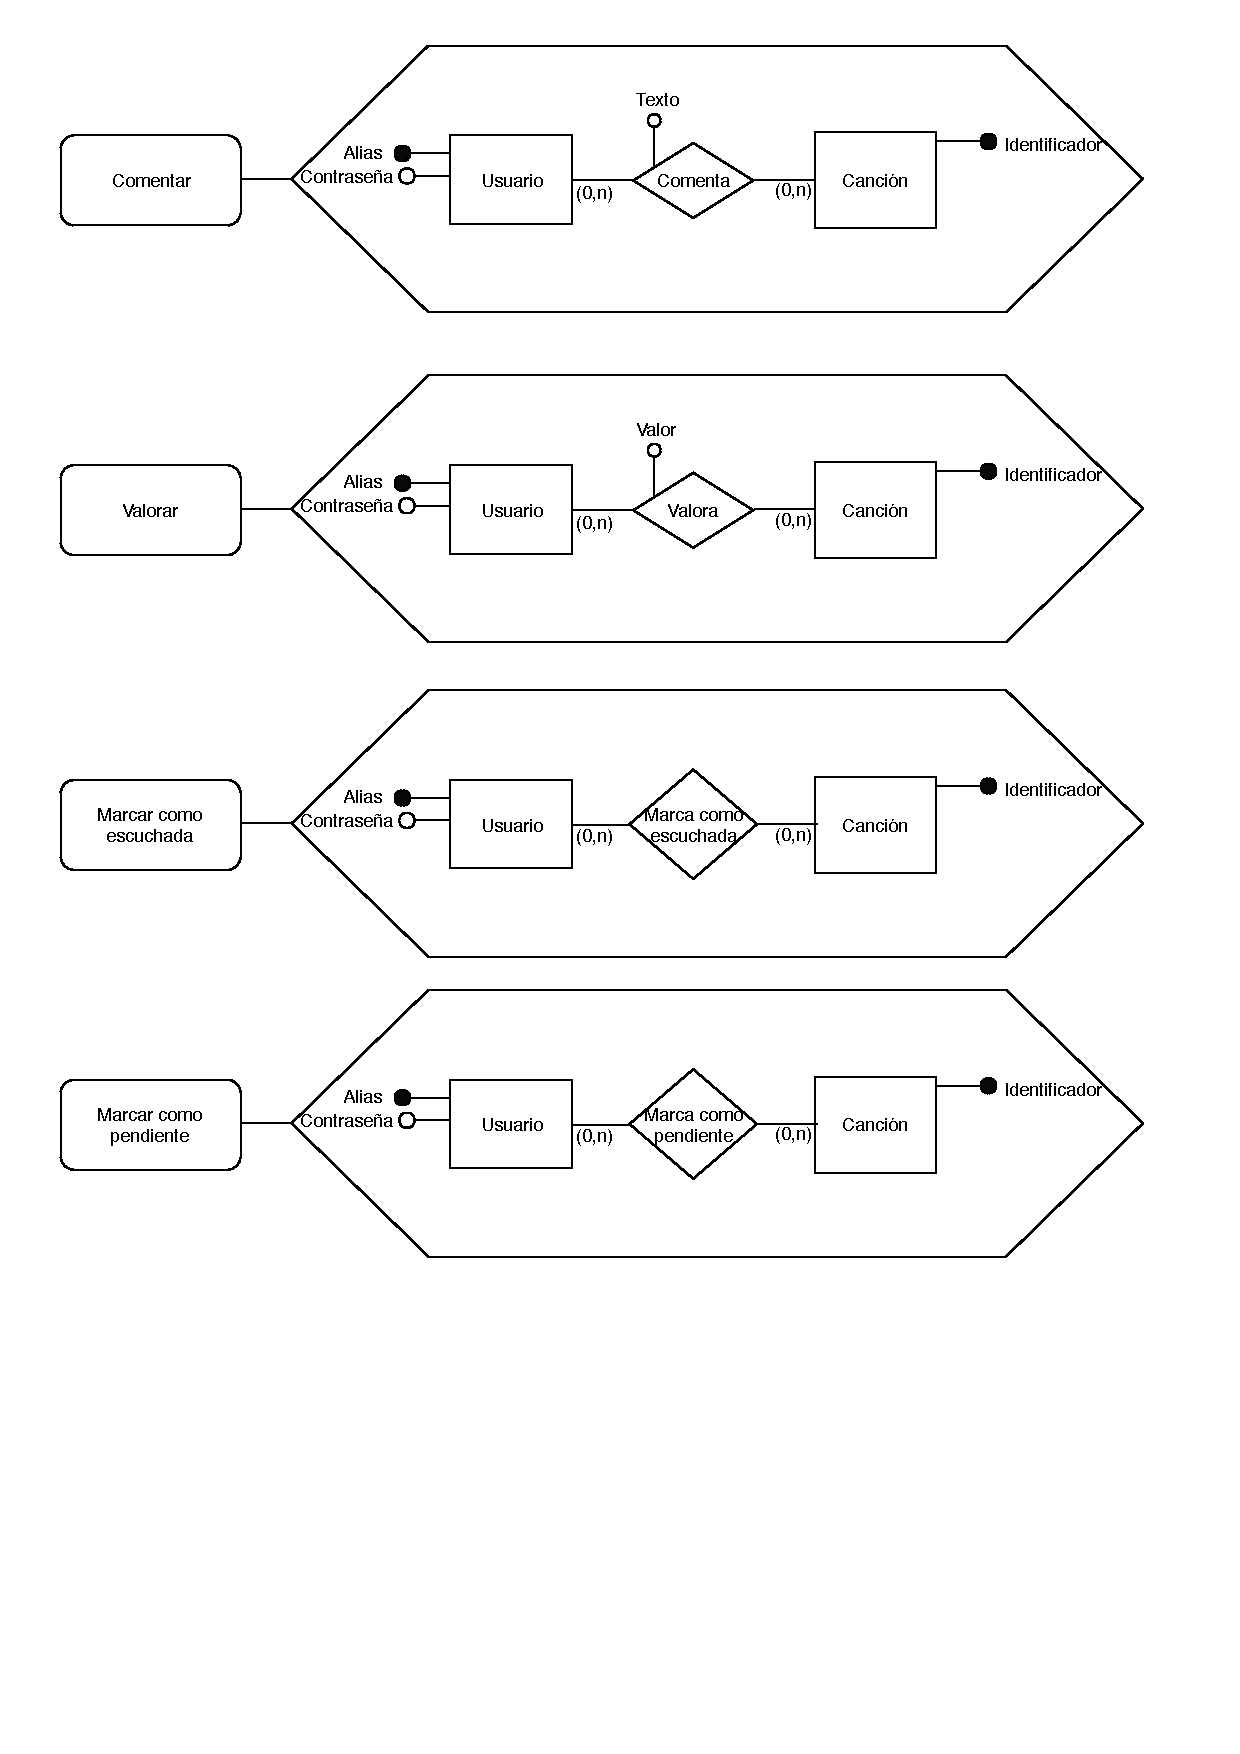
\includegraphics[scale=0.9]{diagramas/Esq-ext-social.pdf}
\end{figure}
\begin{figure}[H]
  \centering
  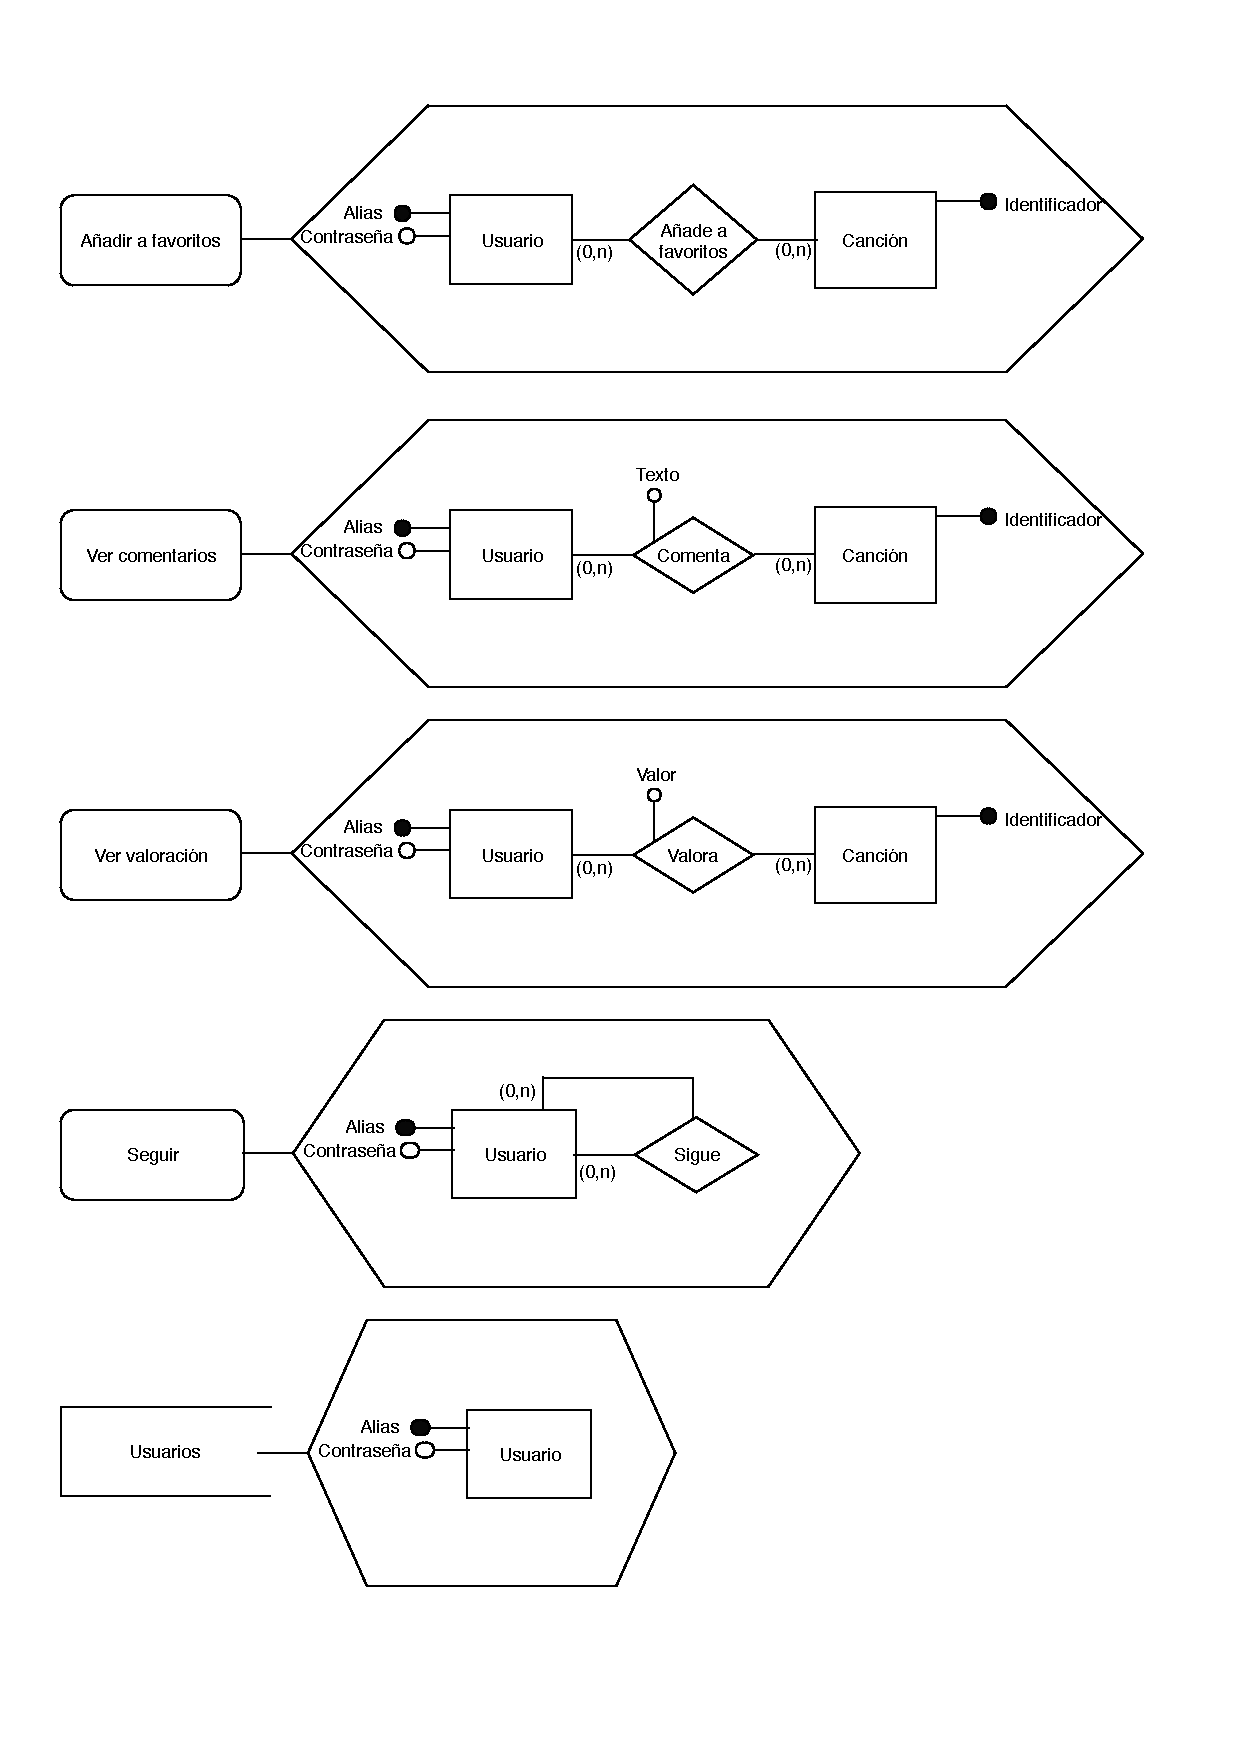
\includegraphics[scale=0.85]{diagramas/Esq-ext-social(1).pdf}
\end{figure}

\begin{figure}[H]
  \caption{Esquemas externos del subsistema de búsquedas y sugerenicas}
  \centering
  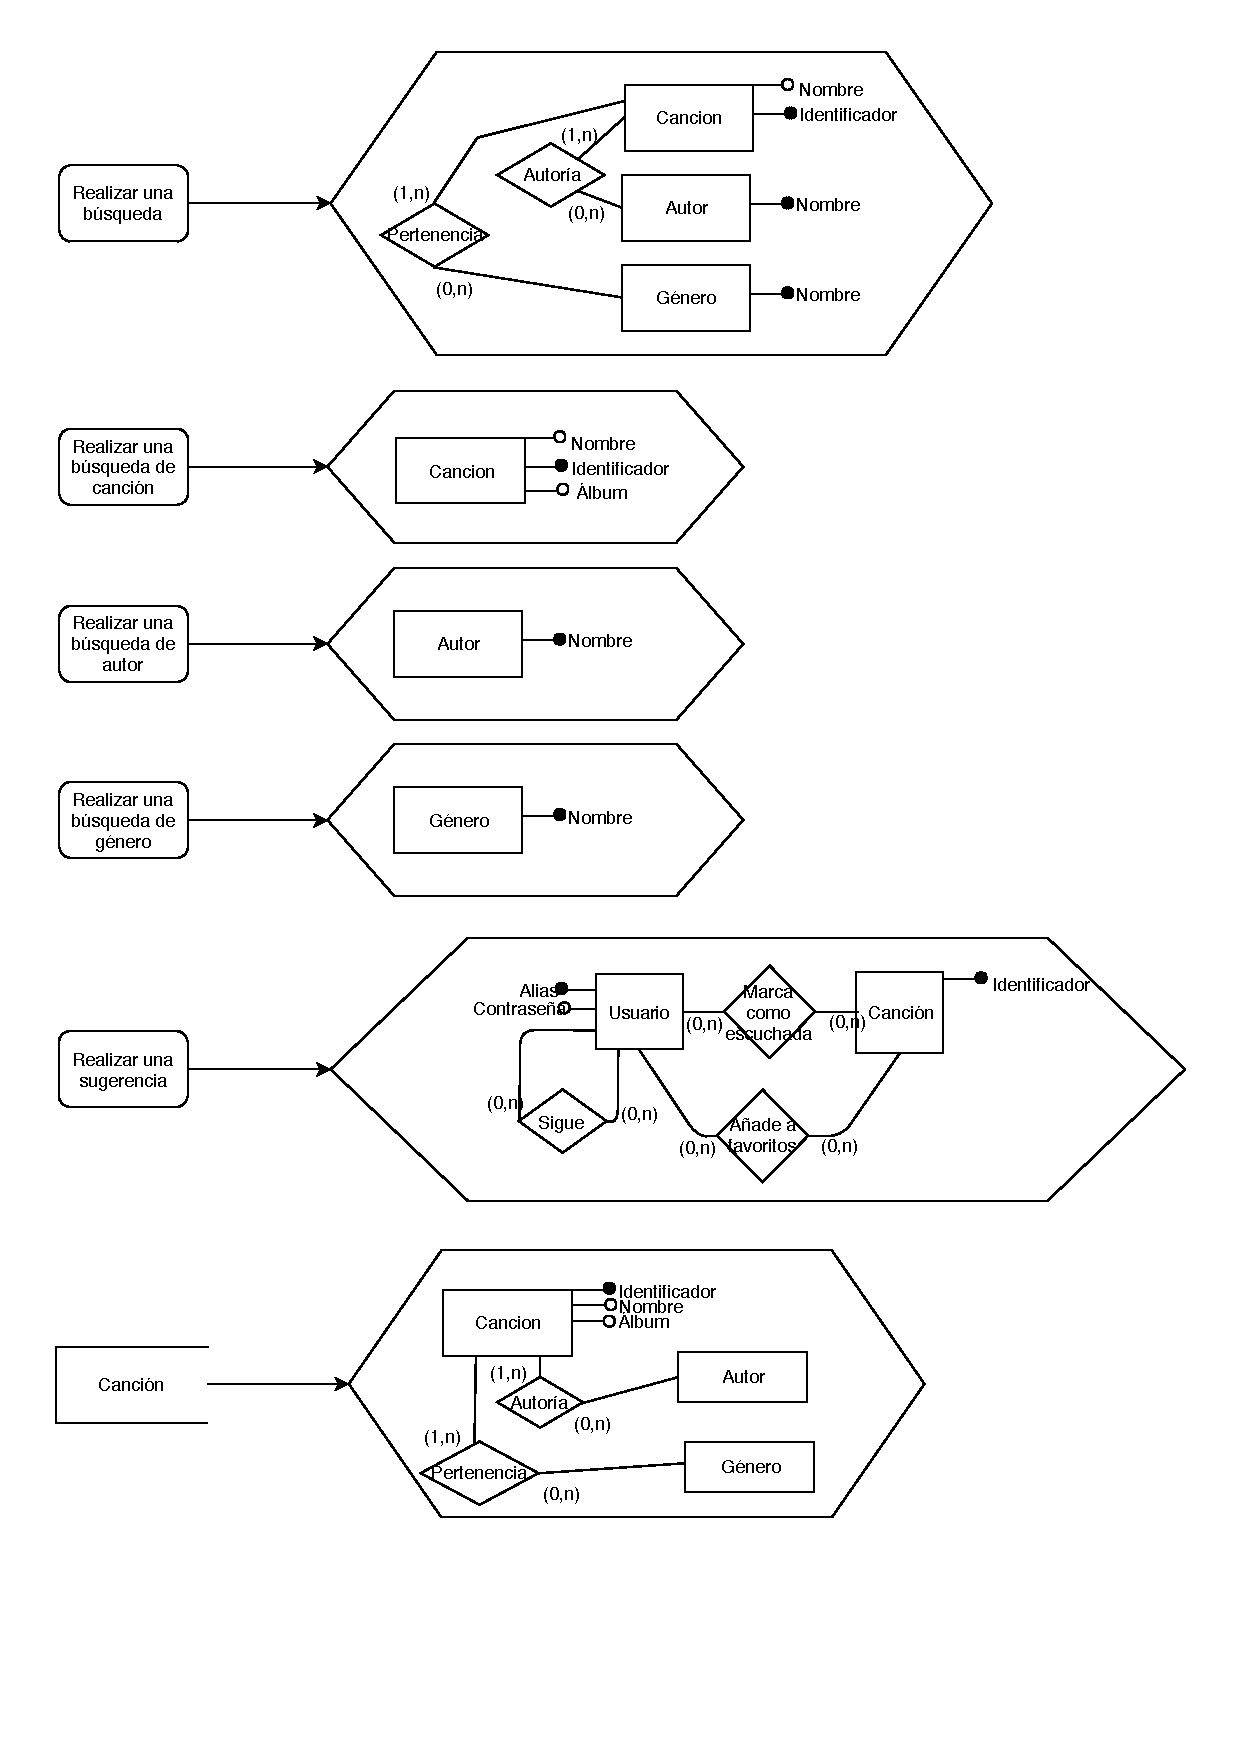
\includegraphics[scale=0.8]{diagramas/busqueda_esquema_externo.pdf}
\end{figure}

\subsection{Diagrama conceptual}

\begin{figure}[H]
  \caption{Diagrama conceptual del subsistema de música}
  \centering
  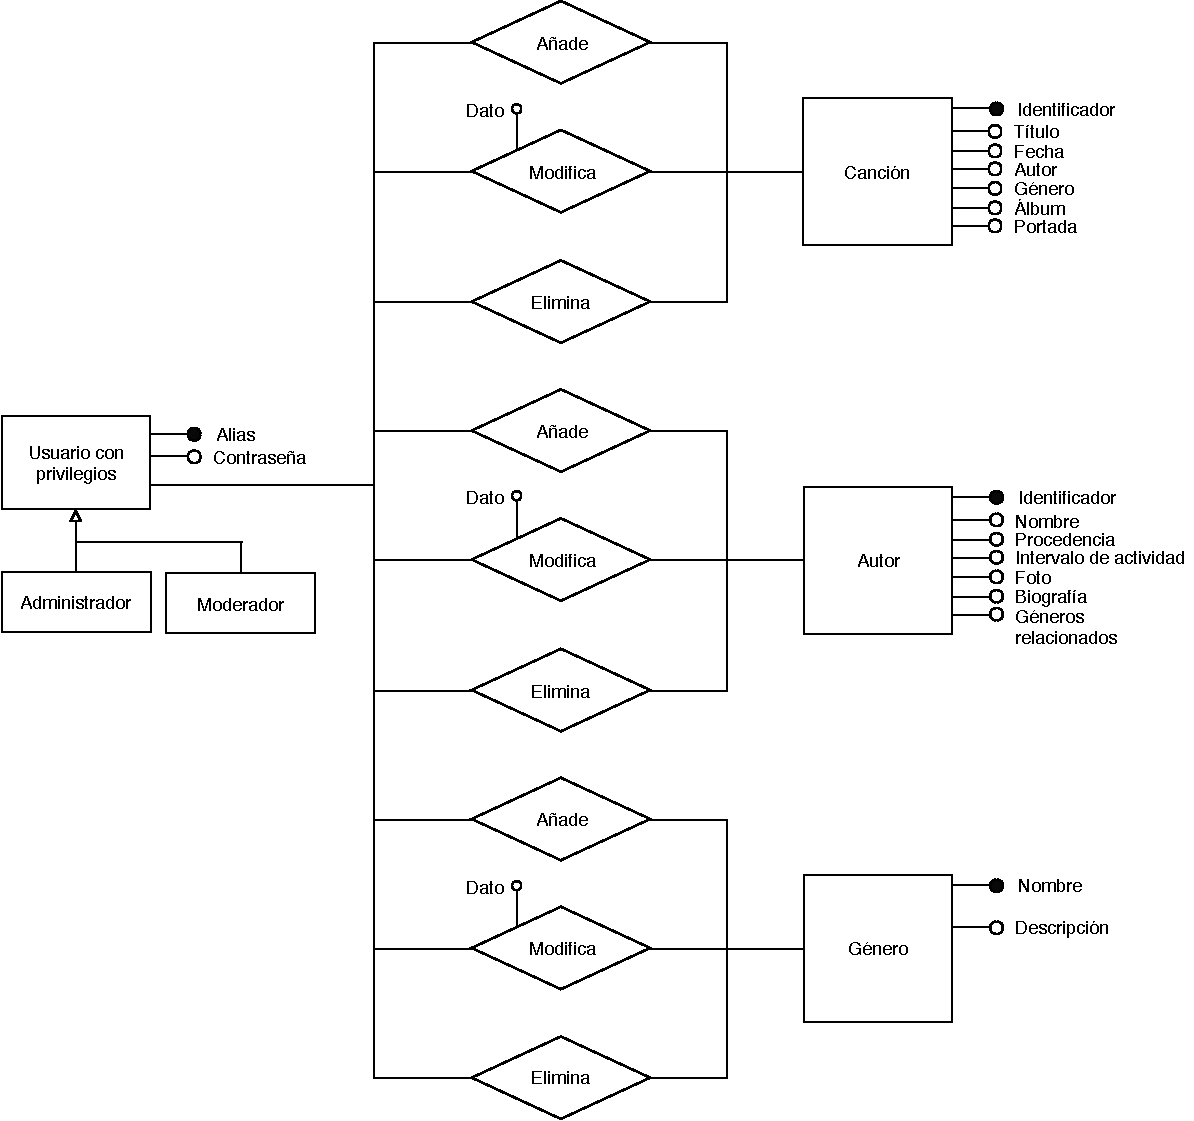
\includegraphics[scale=0.8]{diagramas/musica-conceptual.pdf}
\end{figure}

\begin{figure}[H]
  \caption{Diagrama conceptual del subsistema de usuario}
  \centering
  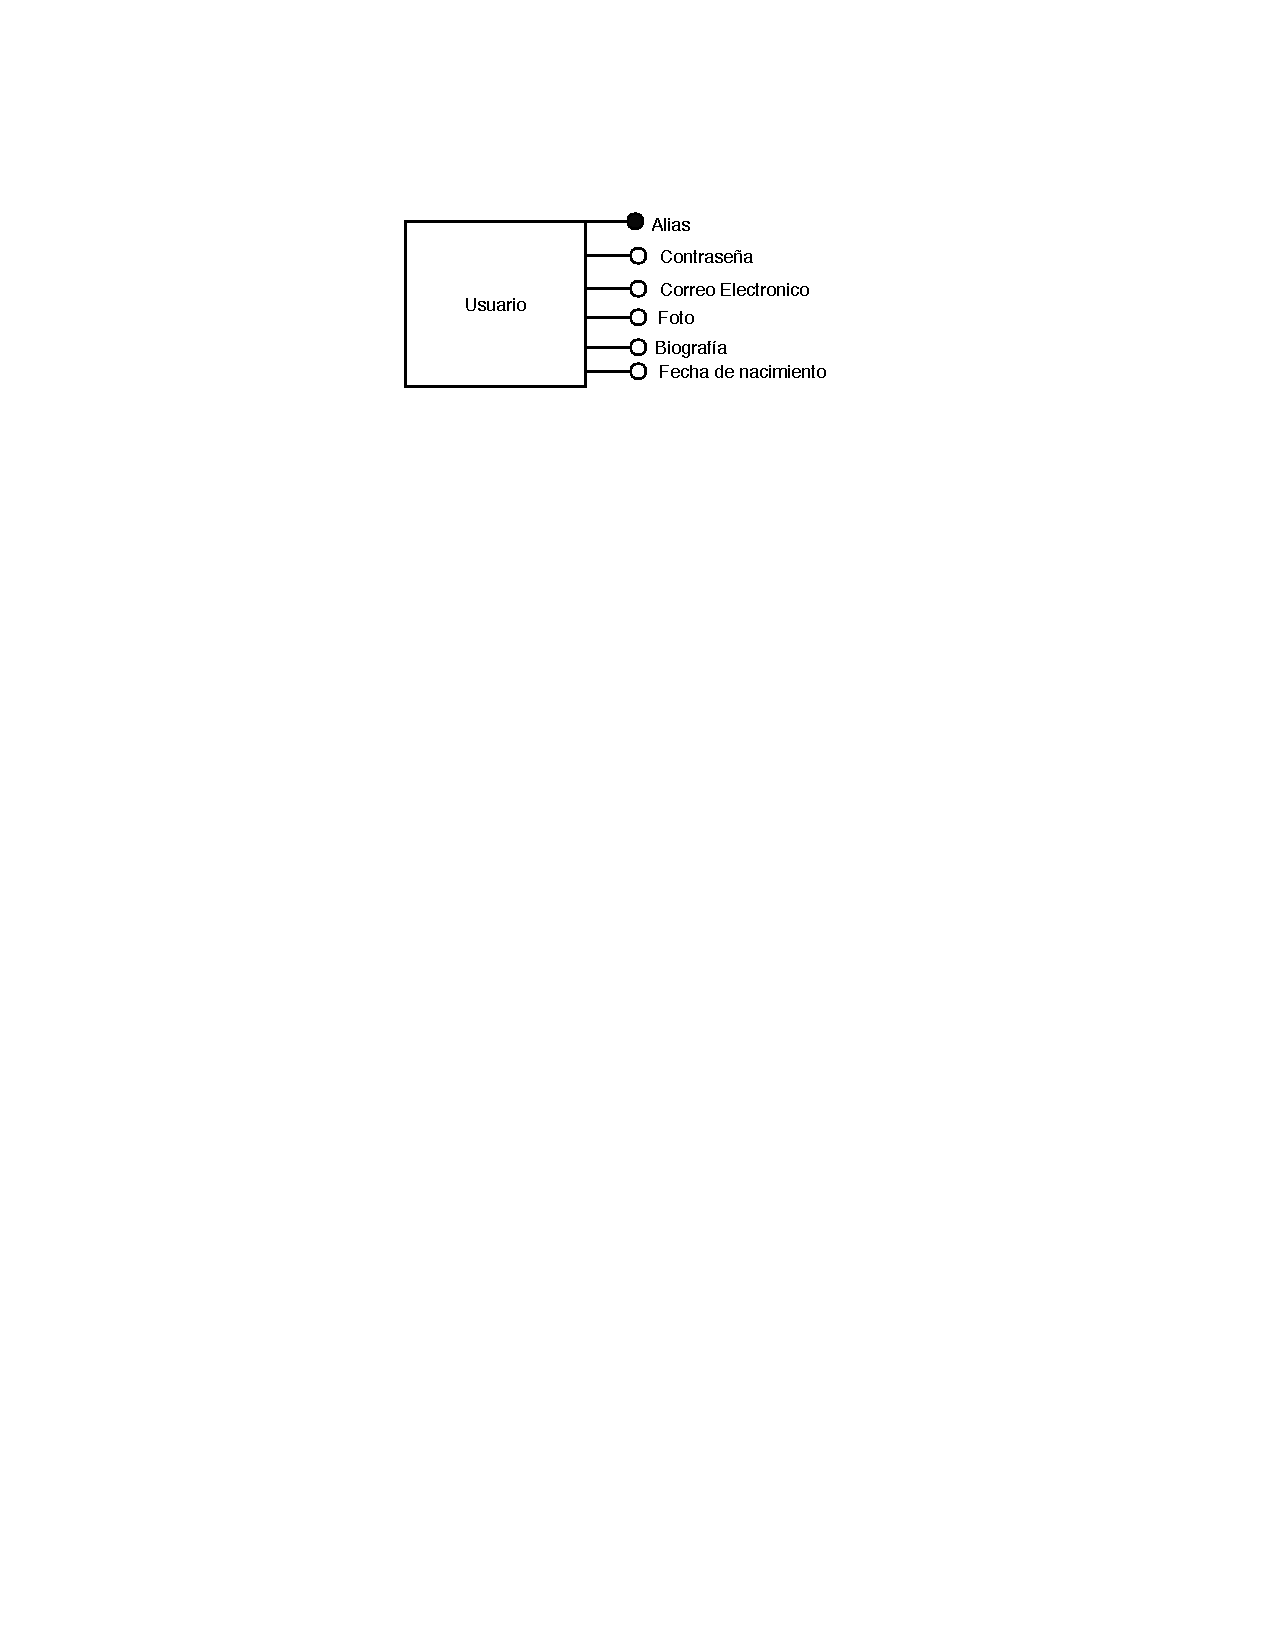
\includegraphics{diagramas/conceptual-usuario.pdf}
\end{figure}

\begin{figure}[H]
  \caption{Diagrama conceptual del subsistema social}
  \centering
  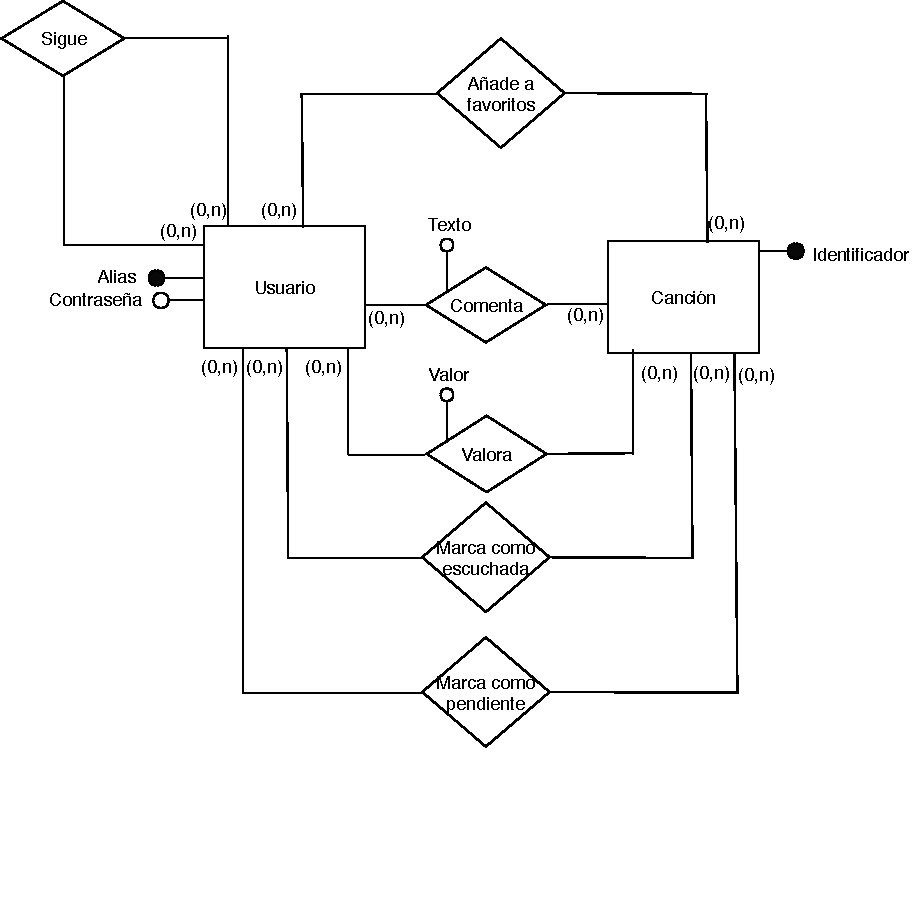
\includegraphics{diagramas/conceptual-social.pdf}
\end{figure}

\begin{figure}[H]
  \caption{Diagrama conceptual del subsistema de búsquedas y sugerencias}
  \centering
  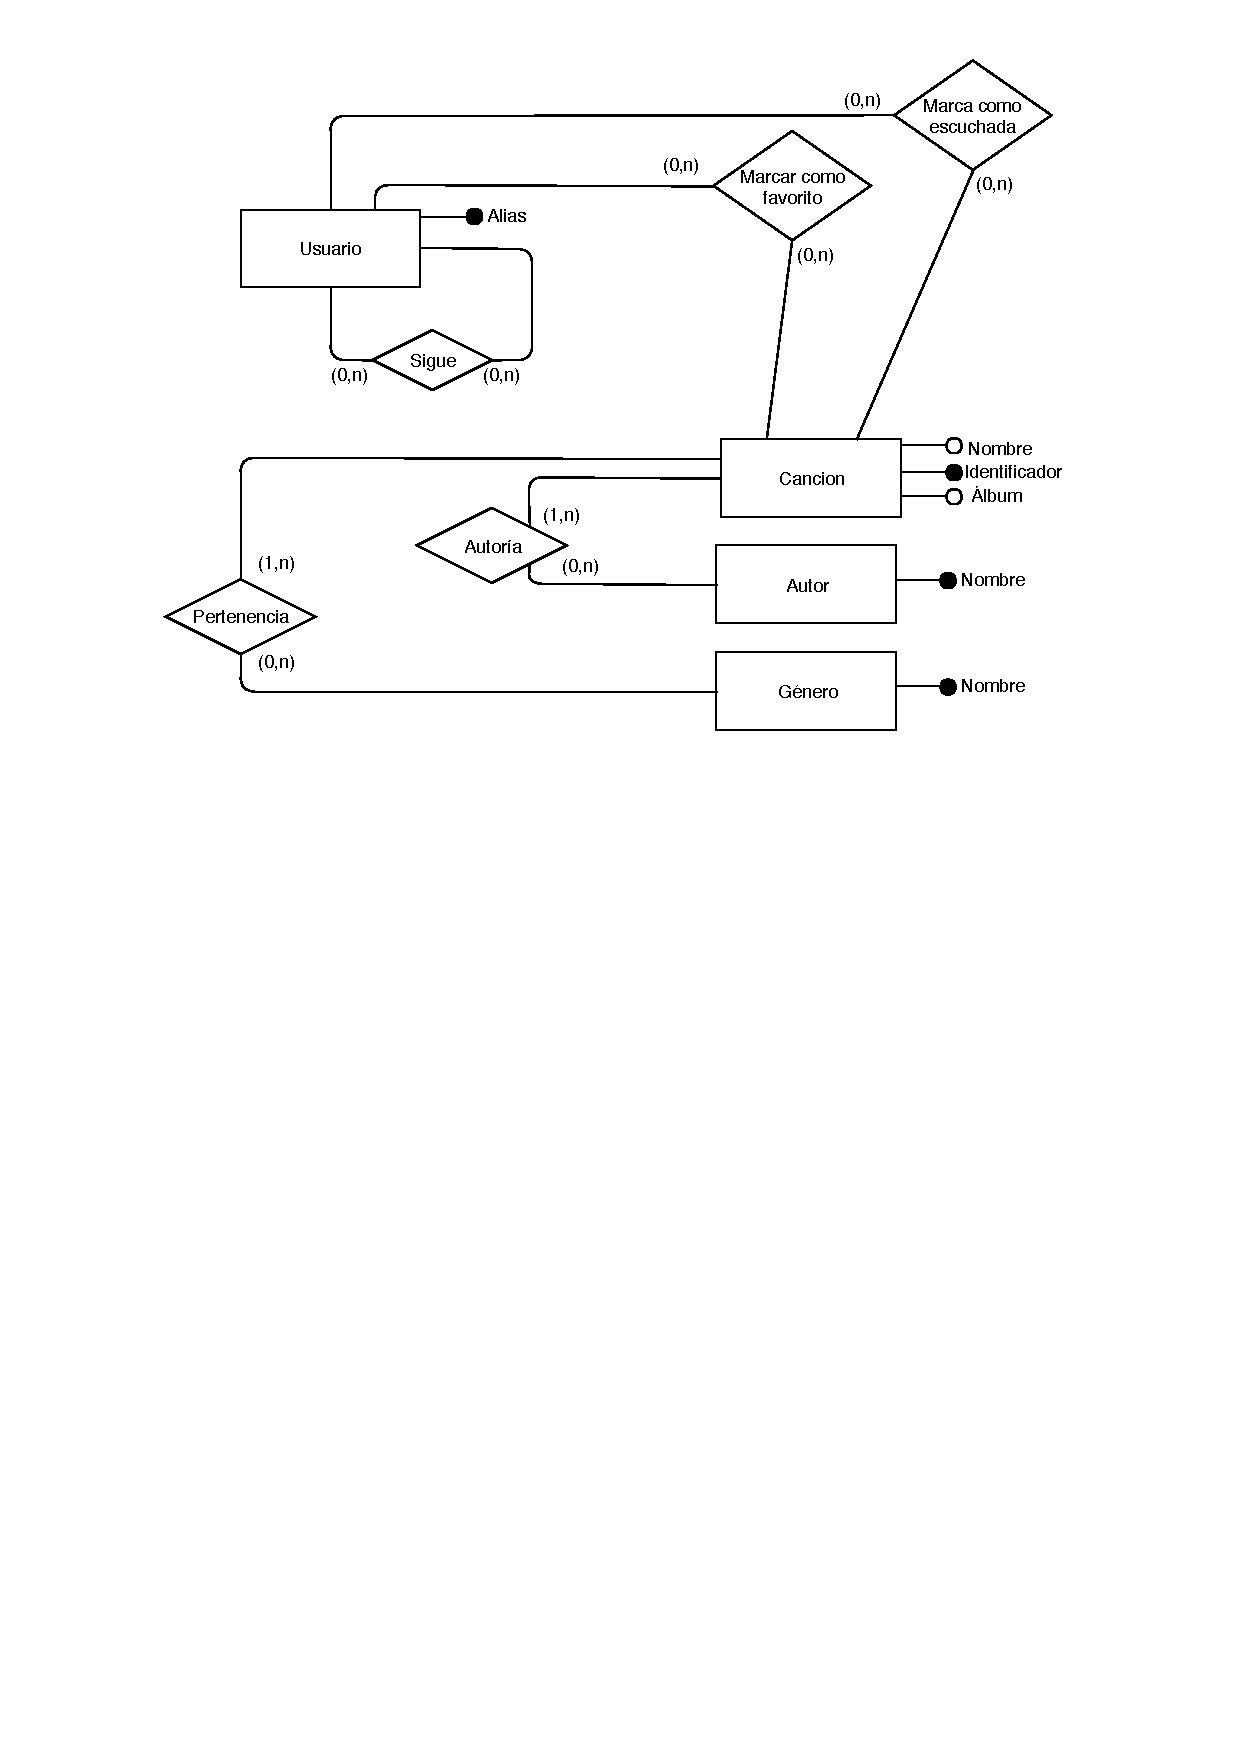
\includegraphics{diagramas/busqueda_modelo_conceptual.pdf}
\end{figure}

\subsection{Modelo entidad/relación}

\begin{figure}[H]
  \caption{Modelo entidad/relación}
  \centering
  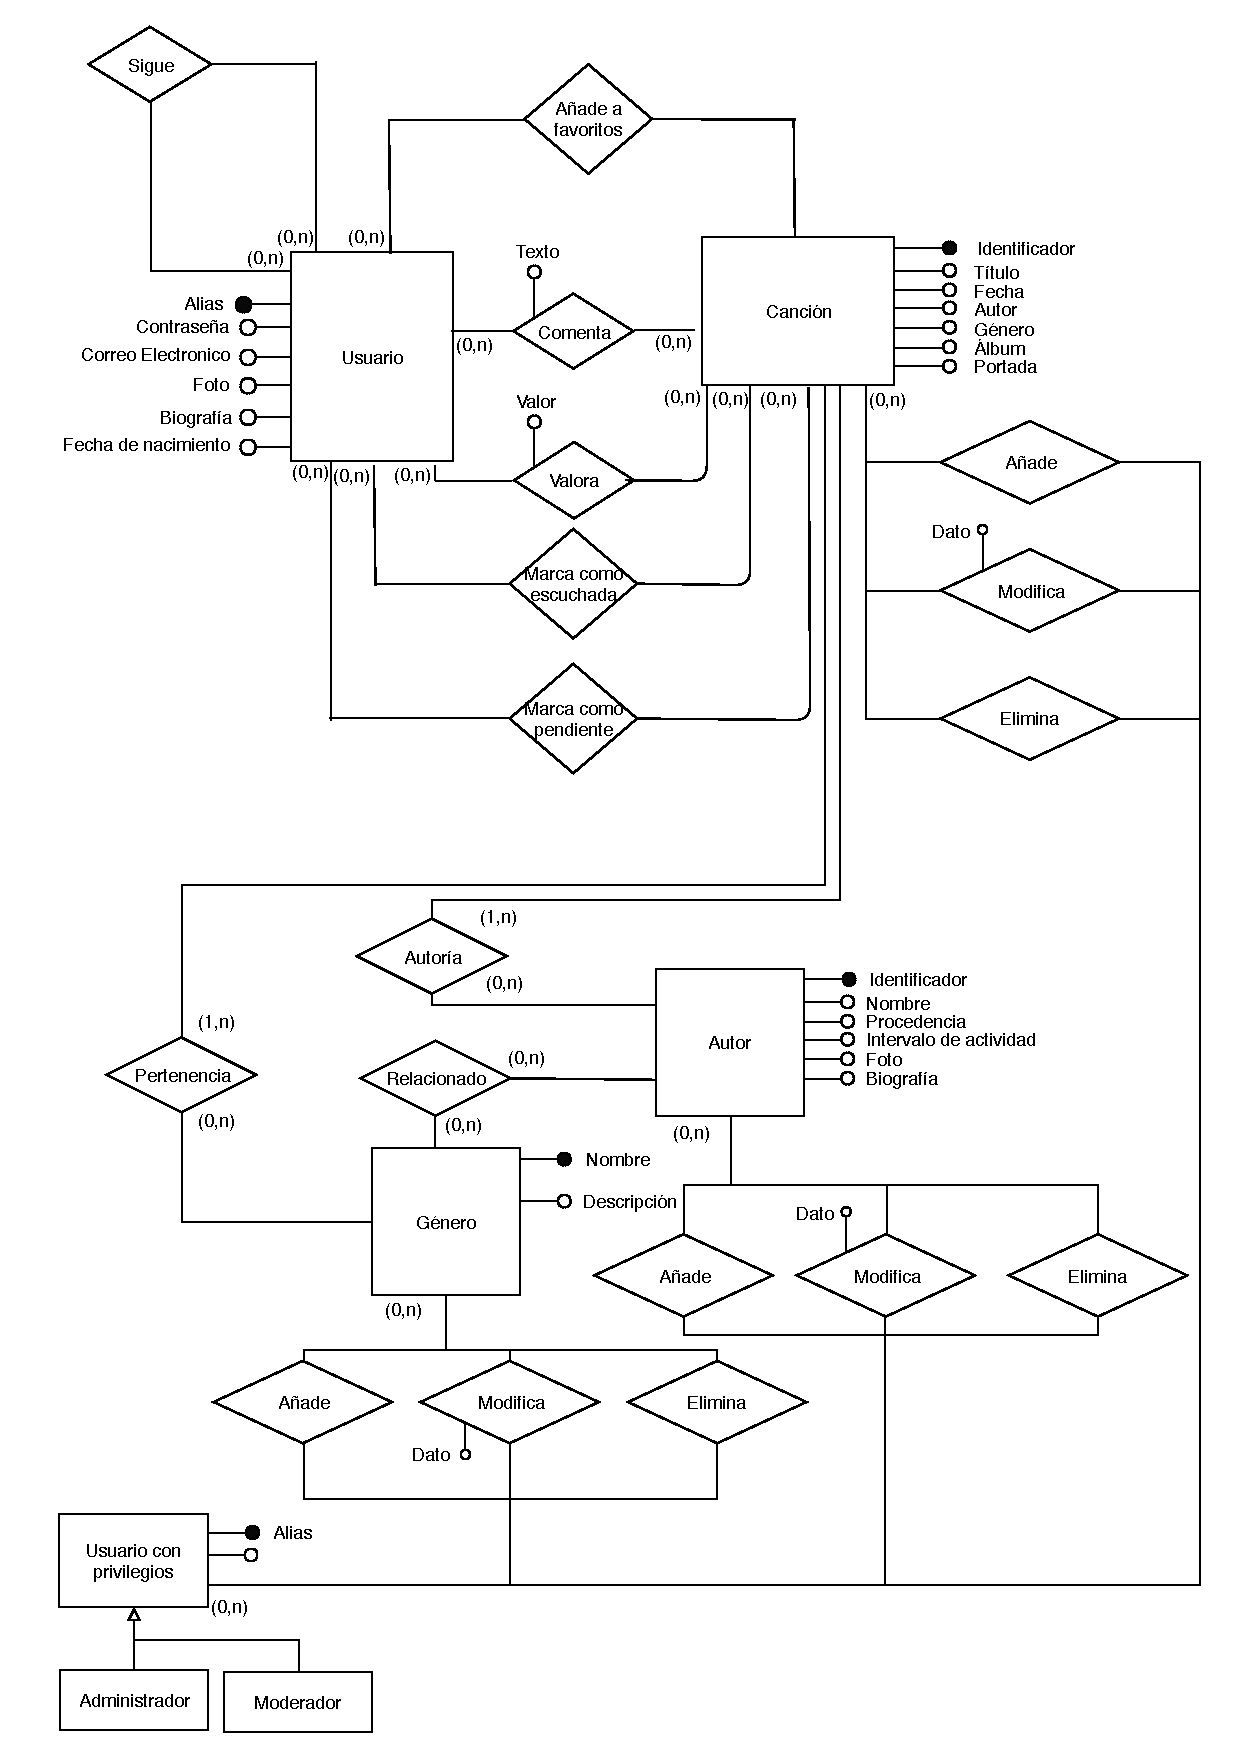
\includegraphics[scale=0.7]{diagramas/modelo-e-r.pdf}
\end{figure}
